%  sample eprint article in LaTeX           --- M. Peskin, 9/7/00
%  modified for LHCP2017, lhcp2017@sjtu.edu.cn
%  This file is part of a tar file, which can be downloaded from the LHCP2017 indico site. 
%   https://indico.cern.ch/event/517784/overview 
% 


\documentclass[10pt]{article}
\usepackage{graphicx}
\usepackage{hyperref}
\usepackage{amssymb}
\usepackage{subcaption}

%particles
\newcommand{\jpsi}{\rm J/$\psi$}
\newcommand{\psip}{$\psi^\prime$}
\newcommand{\jpsiDY}{\rm J/$\psi$\,/\,DY}
\newcommand{\chic}{$\chi_{\rm c}$}
\newcommand{\pip}{$\pi^{+}$}
\newcommand{\pim}{$\pi^{-}$}
\newcommand{\pizero}{$\pi^{0}$}
\newcommand{\kap}{K$^{+}$}
\newcommand{\kam}{K$^{-}$}
\newcommand{\pbar}{$\rm\overline{p}$}
\newcommand{\ccbar}{\ensuremath{\mathrm{c\overline{c}}}}
\newcommand{\bbbar}{\ensuremath{\mathrm{b\overline{b}}}}
\newcommand{\Dzero}{\ensuremath{\mathrm{D^{0}}}}
\newcommand{\Dzerobar}{\ensuremath{\mathrm{\overline{D}^{0}}}}
\newcommand{\Dpm}{\ensuremath{\mathrm{D^{\pm}}}}
\newcommand{\Ds}{\ensuremath{\mathrm{D_{s}^{\pm}}}}
\newcommand{\Dstar}{\ensuremath{\mathrm{D^{*\pm}}}}

%collision systems
\newcommand{\pp}{pp}
\newcommand{\pPb}{p--Pb}
\newcommand{\PbPb}{Pb--Pb}

%detectors
\newcommand{\ezdc}{$E_{\rm ZDC}$}

%units
\newcommand{\GeVc}{GeV/$c$}
\newcommand{\GeVcsq}{GeV/$c^2$}

%others
\newcommand{\degree}{$^{\rm o}$}
\newcommand{\s}{\ensuremath{\sqrt{s}}}
\newcommand{\snn}{\ensuremath{\sqrt{s_{\rm NN}}}}
\newcommand{\y}{\ensuremath{y}}
\newcommand{\pt}{\ensuremath{p_{\rm T}}}
\newcommand{\dedx}{d$E$/d$x$}
\newcommand{\dndy}{d$N$/d$y$}
\newcommand{\dndydpt}{${\rm d}^2N/({\rm d}y {\rm d}p_{\rm t})$}
\newcommand{\zpar}{\ensuremath{z_{||}}}
\newcommand{\zpargen}{\ensuremath{z_{||}^{\mathrm{part}}}}
\newcommand{\zpardet}{\ensuremath{z_{||}^{\mathrm{det}}}}
\newcommand{\ptchjet}{\ensuremath{p_{\mathrm{T,ch\, jet}}}}
\newcommand{\ptjet}{\ensuremath{p_{\mathrm{T,jet}}}}
\newcommand{\ptchjetgen}{\ensuremath{p_{\mathrm{T,ch\,jet}}^{\mathrm{part}}}}
\newcommand{\ptchjetdet}{\ensuremath{p_{\mathrm{T,ch\,jet}}^{\mathrm{det}}}}
\newcommand{\ptd}{\ensuremath{p_{\mathrm{T,D}}}}
\newcommand{\ptdgen}{\ensuremath{p_{\mathrm{T,D}}^{\mathrm{part}}}}
\newcommand{\ptddet}{\ensuremath{p_{\mathrm{T,D}}^{\mathrm{det}}}}
\newcommand{\antikt}{anti-\ensuremath{k_{\mathrm{T}}}}
\newcommand{\Antikt}{Anti-\ensuremath{k_{\mathrm{T}}}}
\newcommand{\kt}{\ensuremath{k_{\mathrm{T}}}}
\newcommand{\pthard}{\ensuremath{p_{\mathrm{T,hard}}}}

%%%%%%%%%%%%%%%%%%%%%%%%%%%%%%%%%%%%%%%%%%%%%%%%%%%%%%%%%%%%%%%%%%%%%%%%%%%%
%   document style macros
%%%%%%%%%%%%%%%%%%%%%%%%%%%%%%%%%%%%%%%%%%%%%%%%%%%%%%%%%%%%%%%%%%%%%%%%%%%%
\def\Title#1{\begin{center} {\Large #1 } \end{center}}
\def\Author#1{\begin{center}{ \sc #1} \end{center}}
\def\Address#1{\begin{center}{ \it #1} \end{center}}
\def\andauth{\begin{center}{and} \end{center}}
\def\submit#1{\begin{center}Submitted to {\sl #1} \end{center}}
\newcommand\pubblock{\rightline{\begin{tabular}{l} Proceedings of the Fifth Annual LHCP\\ \pubnumber\\
         \pubdate  \end{tabular}}}

\newenvironment{Abstract}{\begin{quotation} \begin{center} 
             \large ABSTRACT \end{center}\bigskip 
      \begin{center}\begin{large}}{\end{large}\end{center} \end{quotation}}

\newenvironment{Presented}{\begin{quotation} \begin{center} 
             PRESENTED AT\end{center}\bigskip 
      \begin{center}\begin{large}}{\end{large}\end{center} \end{quotation}}

\def\Acknowledgements{\bigskip  \bigskip \begin{center} \begin{large}
             \bf ACKNOWLEDGEMENTS \end{large}\end{center}}
%%%%%%%%%%%%%%%%%%%%%%%%%%%%%%%%%%%%%%%%%%%%%%%%%%%%%%%%%%%%%%%%%%%%%%%%%%%%
%  personal abbreviations and macros
%    the following package contains macros used in this document:
\input econfmacros.tex
%%%%%%%%%%%%%%%%%%%%%%%%%%%%%%%%%%%%%%%%%%%%%%%%%%%%%%%%%%%%%%%%%%%%%%%%%%%

\textwidth=6.5in  \textheight=8.75in
\hoffset=-.85in
\voffset=-0.6in

%%  DO NOT CHANGE anything above.

% include packages you will need
\usepackage{color}

%%%%%%%%%%%%%%%%%%%%%%%%%%%%%%%%%%%%%%%%%%%%%%%%%%%%%%%%%%%%%%%%%%%%
% basic data for the eprint:
%%%%%%%%%%%%%%%%%%%%%%%%%%%%%%%%%%%%%%%%%%%%%%%%%%%%%%%%%%%%%%%%%%%%

% Instruction:
% Please change each of the following fields:
%

%% preprint number data:
% If there is a preprint number from your institute, or experiment note number, please fill it in 
%\newcommand\pubnumber{ ATL-PHYS-PROC-2017-XXX }
\newcommand\pubnumber{ }

%% date
\newcommand\pubdate{\today}

%%  Affiliation
\def\affiliation{
On behalf of the ALICE Collaboration, \\
Physics Department, Yale University, New Haven, CT 06511, USA}

%% Acknowledge the support
\def\support{\footnote{Work supported by the U.S. Department of Energy under grant number DE-SC0004168.}}

\begin{document}

% large size for the first page
\large
\begin{titlepage}
\pubblock


%% Change the title, name, abstract
%% Title 
\vfill
\Title{New results on jets and heavy flavor in heavy-ion collisions with ALICE}
\vfill

%  if you need to add the support use this, fill the \support definition above. 
%   \Author{ FIRSTNAME LASTNAME \support }
\Author{Salvatore Aiola\support}
\Address{\affiliation}
\vfill
\begin{Abstract}

here it goes

\end{Abstract}
\vfill

% DO NOT CHANGE 
\begin{Presented}
The Fifth Annual Conference\\
 on Large Hadron Collider Physics \\
Shanghai Jiao Tong University, Shanghai, China\\ 
May 15-20, 2017
\end{Presented}
\vfill
\end{titlepage}
\def\thefootnote{\fnsymbol{footnote}}
\setcounter{footnote}{0}
%

% normal size for the rest
\normalsize 

%% Your paper should be entered below. 

\section{Introduction}
A comprehensive and far-reaching heavy-ion programme is part of the scientific goals of the CERN Large Hadron Collider.
The large statistics accumulated during the LHC Run-1 and Run-2 have given access to an unprecedented number of observables connected to rare high-$Q^2$ processes.
Such hard probes are rare enough to be singled out from the large bulk of particles produced in ultra-relativistic heavy-ion collision. By interacting with the Quark-Gluon Plasma (QGP) these self-produced probes
become carriers of crucial pieces of information about the transport properties of the QGP.

The suppression of the jet production cross section in ultra-relativistic heavy-ion collisions has been established both at RHIC~\cite{STAR:2017a} and at the LHC~\cite{ALICE:2015a}. The suppression is interpreted as the result of the interaction of the hard-scattered partons 
with the QGP, which dampens the momentum of the hard parton via radiative and collisional energy loss (\emph{jet quenching}). A number of theoretical models, such as JEWEL and YaJEM, can effectively reproduce
the data; however the exact determination of the parameters of the energy loss as well as the details of the energy-loss mechanism are still pending. Some additional constraints come from the observation (or lack thereof) of
the modification of the internal structure of the jets. A number of observable has been proposed. The ALICE Collaboration is active in this area and some of the latest results have been presented at this conference.

Heavy-flavor (charm and beauty) particles have been used as probes of the QGP both at RHIC and at the LHC. What makes heavy-flavor partons special is their non-zero mass which plays the role of a second hard scale, independent of the momentum.
As a consequence, perturbative Quantum Chromo-Dynamics (pQCD) methods are effective in calculating the production cross-section in vacuum, i.e. in \pp\ collisions, down to zero momentum, notwithstanding large uncertainties.
Furthermore the non-zero mass of charm and beauty has an impact in their interaction with the QGP, which have been investigated both theoretically~\cite{} and experimentally~\cite{}. 
Therefore studying the dynamics of heavy quarks in the QGP can put important additional constraints on its transport properties.
At this conference the ALICE Collaboration has presented an updated measurement of the $v_2$ of D mesons as well as \jpsi, using the larger statistical samples available from Run-2.

In recent years, collective effects usually associated with the formation of the QGP have been observed in a subset of \pPb\ and in \pp\ collisions, characterised by a very large event multiplicity. These observations could be taken as indication that the smallest drop
of QGP is formed in such collisions, however no unambiguous proof has been shown yet. In particular no unexpected effects have been observed using hard probes (jets or heavy-flavor particles). In these proceedings we present two recent measurements from ALICE.

The ALICE detector and its performance are described elsewhere~\cite{}. We refer the interested reader to those publications.

\section{\PbPb\ collisions}

\subsection{Jet Substructure}
If two partons within the same parton shower are separated by a distance smaller than the tranvserse resolution scale of the medium, they interact coherently with the QGP as a color singlet (color coherence). 
Conversely, if they are separated by larger distances they interact incoherently with the medium as independent color charges.
The transverse resolution scale can be characterized with a critical angle $\theta_{\rm c}$. This angle can be related to the medium decoherence parameter $\Delta_{\rm med}$, which enters the amplitude of the antenna emission, via Eq.~\ref{eq:delta_med}\cite{Mehtar-Tani:2012, Casalderrey-Solana:2013}.
\begin{equation}
\Delta_{\rm med} \simeq 1 - e^{-\frac{1}{12}\hat{q}Lr^2_{\bot}} \equiv 1 - e^{-(\theta/\theta_{\rm c})^2}
\label{eq:delta_med}
\end{equation}
Here $\hat{q}$ is the medium transport parameter, $L$ is the medium's
length and $r_{\bot}$ is the jet's transverse extension in the medium. $\theta$ is the jet's opening angle, which is given by
the largest antenna (the two substructures with the largest angular separation) in the jet which in a vacuum
corresponds to the first splitting. Recent theoretical work has highlighted the sensitivity of two-pronged jets
to coherence effects in the QGP~\cite{}.

The nsubjettiness~\cite{} $\tau_{\rm N}$ is a measure of how $N$-cored a jet's substructure is. It is defined in Eq.~\ref{eq:nsubjettiness}, where
$i$ denotes each jet constituents, $N$ is the number of cores found in the jet, $M$ is the number of jet constituents, $R$ is the jet resolution parameter used in the \kt\ jet finding algorithm
and $\Delta R_{j,i}$ is the distance in the $(\eta,\phi)$ plane between the track $i$ and the jet axis core $j$.
\begin{equation}
\tau_N = \frac{\sum^M_{i=1}p_{{\rm T},i}\min(\Delta R_{1,i},\Delta R_{2,i},...,\Delta R_{N,i})}{\sum^M_{i=1}p_{{\rm T},i}R}
\label{eq:nsubjettiness}
\end{equation}
A jet with $\tau_N$ approaching $0$ 
has $N$ or fewer definite cores; conversely a $\tau_N$ value
approaching unity indicates the presence of at least $N + 1$ substructures. 
It follows that the ratio $\tau_2/\tau_1$ is sensitive to jets that have exactly two definite hard cores. 

Jets are first reconstructed with the \antikt\ algorithm as implemented in the \texttt{FastJet}\cite{} software package.
Tracks with $p_{\rm T}>0.15$~\GeVc\ and $|\eta|<0.9$ identified in the central tracking system (Inner Tracking System and Time Projection Chamber, see~\cite{}) 
are used for jet reconstruction (\emph{charged jets}). 
Identified jets are reclustered using the exclusive-$k_{\rm T}$ algorithm. In order to obtain the two antenna axes of the jet (first splitting in vaccum) 
the last step in the clustering procedure is unwinded.
The average uncorrelated background is subtracted from the measured nsubjettiness with a constituent subtraction~\cite{} and cross-checked with second oder derivative subtraction~\cite{}, which gives similar results~\cite{}.
A PYTHIA6+GEANT3 simulation is used to estimate the detector effects on the jet \pt\ and on $\tau_2/\tau_1$ and a correction is applied using the 2D Bayesian method~\cite{}.
The hadron-jet coincidence technique described in~\cite{} is used to reject combinatorial jets from the measured sample. 
Instead of the absolute cross section, which suffers from a large combinatorial contamination, the difference in the yields of jets recoiling from two high-\pt\ trigger hadron classes is reported. 
The trigger hadron \pt\ classes are $15-45$~\GeVc\ (signal class) and $8-9$~\GeVc\ (reference class). The distribution of $\tau_2/\tau_1$ is shown in Fig.~\ref{fig:nsubjettiness} for jets with $40<p_{\rm T,ch.jet}<60$~\GeVc.
The measured distribution is compared with a PYTHIA6 Perugia-11 simulation which agrees with the data within the uncertainties. We conclude that no coherence effects in the parton energy loss are supported by this measurement.
\begin{figure}[tb]
\centering
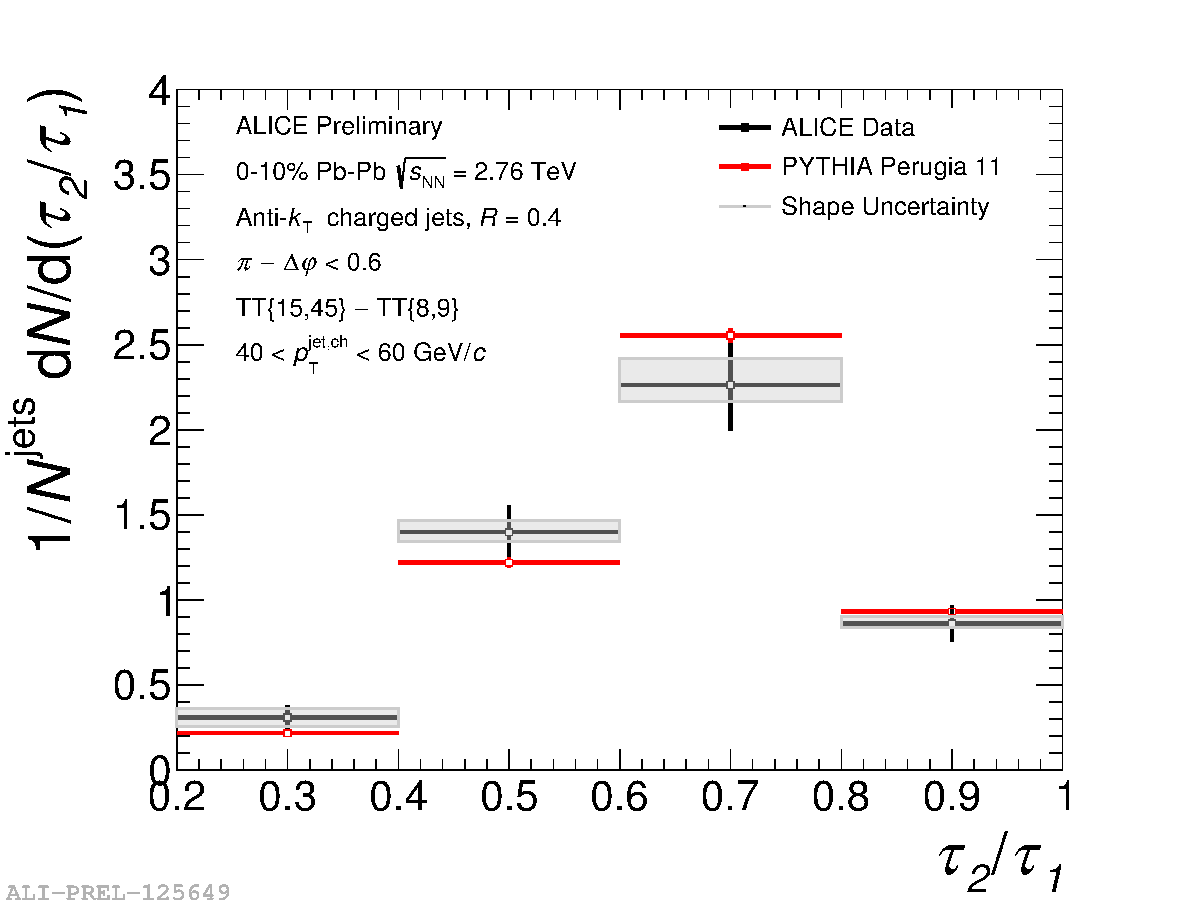
\includegraphics[width=.5\textwidth]{img/2017-Feb-03-Tau2to1_40to60_Full_Results_0}
\caption{Distribution of $\tau_2/\tau_1$ for \antikt\ charged jets with $R=0.4$s in \PbPb\ collisions at $\snn=2.76$~TeV in the $0-10$\% most central events. 
ALICE data points (black) are compared with a PYTHIA6 Perugia-11 simulation (red).}
\label{fig:nsubjettiness}
\end{figure}

ALICE has recently measured the jet mass both in \pPb\ and \PbPb\ collisions. Also for this jet shape observable no modification due to either cold or hot nuclear matter effects is observed~\cite{}.

\subsection{Heavy-Flavor Elliptic Flow}
The azimuthal anisotropy of D mesons is characterized by $v_2= \left<\cos 2(\phi - \psi_2)\right>$, where $\phi$ is the D-meson azimuthal angle and $\psi_2$ is the symmetry plane of the second-order
harmonic in the Fourier decomposition of the azimuthal distribution of the particles produced in the event.
This coefficient is usually referred to as \emph{elliptic flow} because its existence is ascribed to the initial asimmetric spatial configuration of the QGP that is formed in semi-central heavy-ion collisions.
The QGP flows according to pressure gradients which are determined by its almond-like shape.
The measurement of the elliptic flow of D mesons provides important insight into the interactions of charm quarks with the
medium. At low \pt, the D-meson $v_2$ offers the unique opportunity to test whether also charm quarks participate in
the collective expansion dynamics and possibly thermalize in the medium~\cite{}. At high \pt, it provides constraints on the path-length dependence of parton energy loss~\cite{}.
The measurement of the $v_2$ of D mesons has played an important role in challenging
the theoretical models, so it is paramount to measure it with the best precision possible.
Figure~\ref{fig:v2d0} shows the elliptic flow of D mesons in semi-central \PbPb\ collisions at $\snn=5.02$~TeV.
The values of $v_2$ are compatible with the corresponding values for pions within uncertainties in the range $2<\pt<24$~\GeVc.
\begin{figure}[tb]
\centering
\begin{subfigure}[b]{0.43\textwidth}
  \centering
  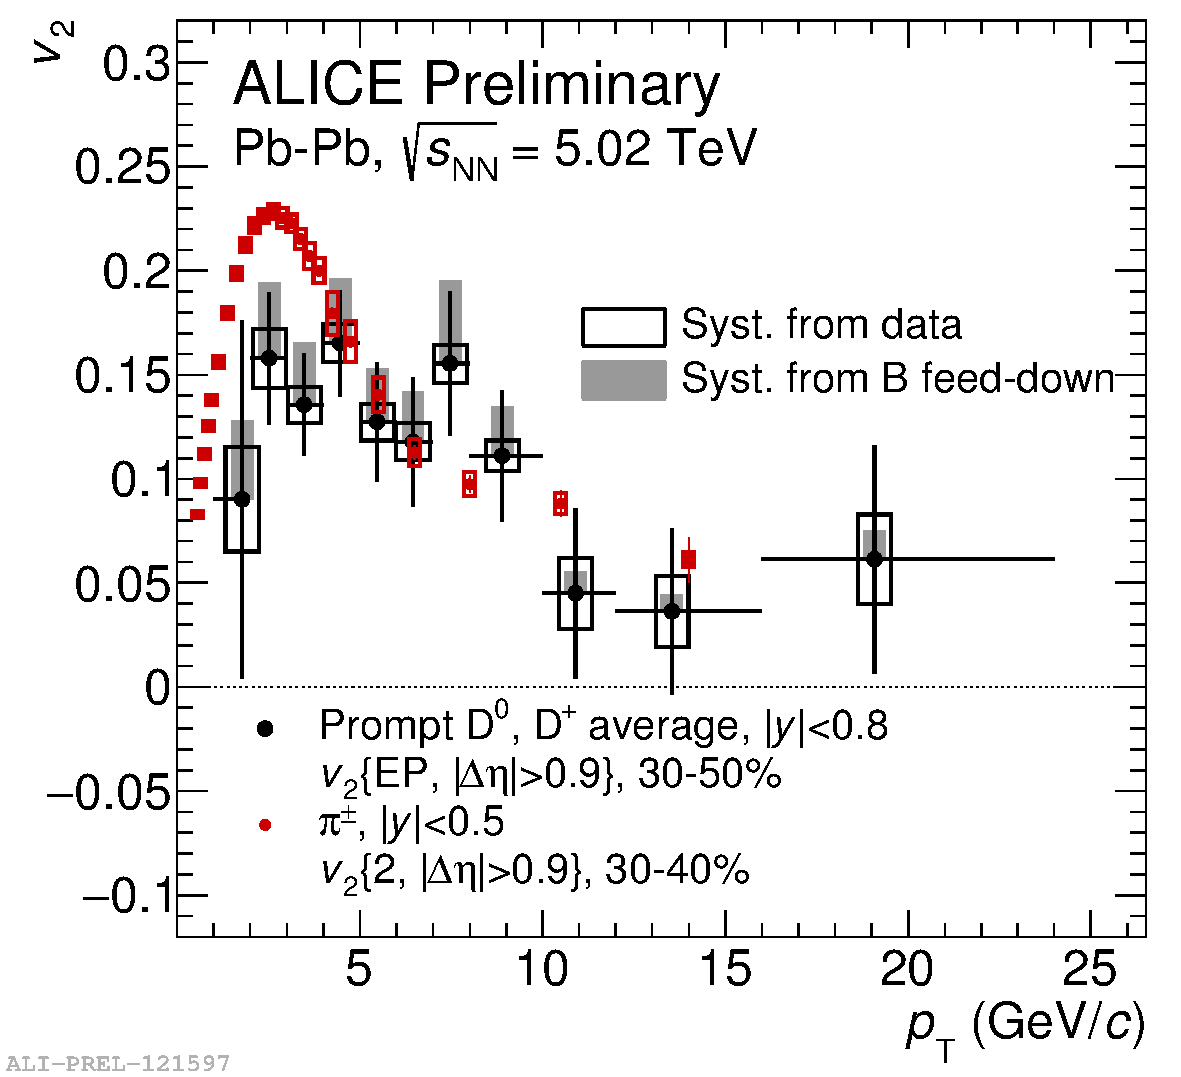
\includegraphics[width=1.0\linewidth]{img/2017-Feb-02-D0DplusAveragev2_Comparison_with_pions_3040}
  \caption{D meson vs. pion elliptic flow.}
  \label{fig:v2d0}
\end{subfigure} \quad
\begin{subfigure}[b]{0.53\textwidth}
  \centering
  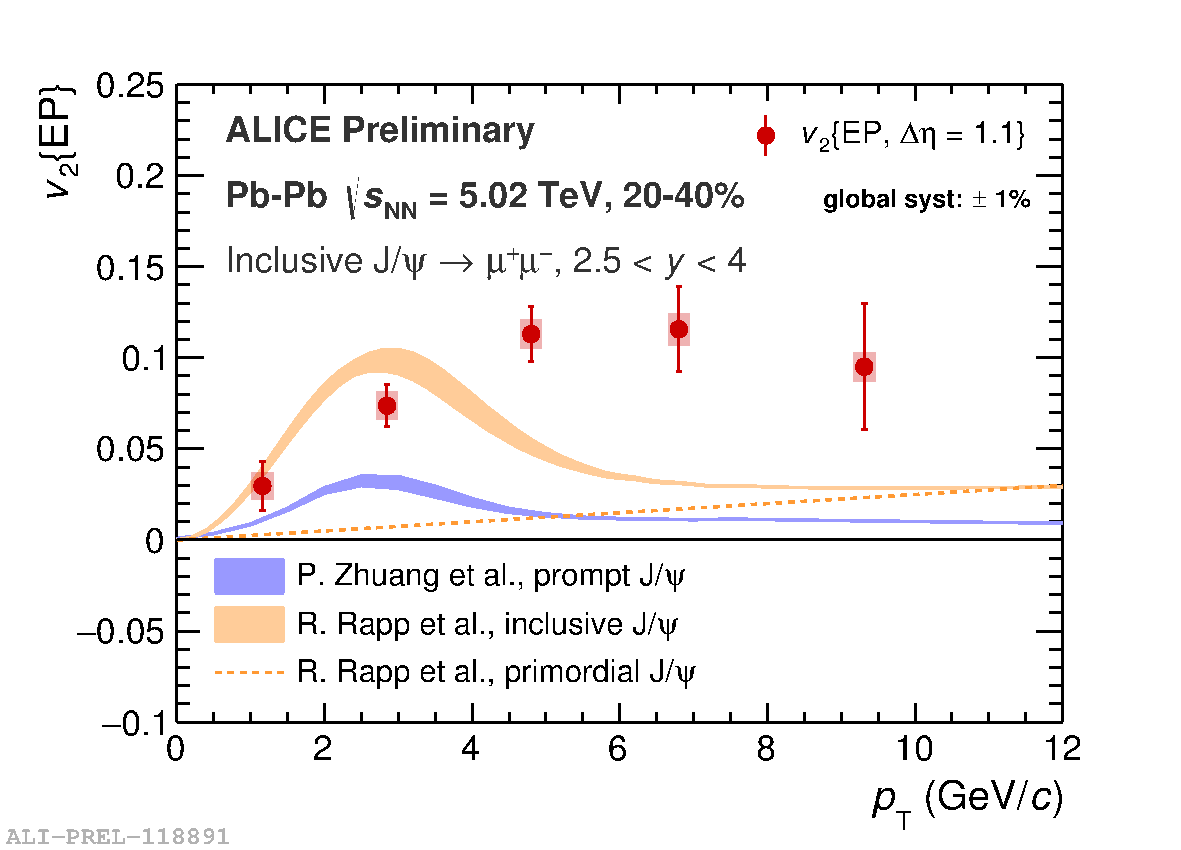
\includegraphics[width=1.0\linewidth]{img/2017-Feb-03-jpsiv2_theory}
  \caption{\jpsi\ elliptic flow}
  \label{fig:v2jpsi}
\end{subfigure} \quad
\caption{Left: elliptic flow of \Dzero\ mesons (black) compared with the elliptic flow of pions (red) in semi-central \PbPb\ collisions at $\snn=5.02$~TeV. Right: elliptic flow of \jpsi\ (red) compared with theoretical calculations in the same collision system.}
\end{figure}

Hidden-charm mesons have an equally important role in the characterisation of the QGP.
The observed \jpsi\ yield in heavy-ion collision has been interpreted as being the result of two competing effects: dissociation of the \ccbar\ pairs in the QGP; and generation in the QGP from pairs of charm and anti-charm quarks coming from initially independent hard scatterings.
The \jpsi\ mesons generated in the QGP are expected to flow with the QGP medium. The strong $v_2$ of \jpsi, shown in Fig.~\ref{fig:v2jpsi} is an indication of large fraction of \jpsi\ generated in the QGP.

\section{\pPb\ collisions}

\subsection{Hadron-Jet Cross Section}

\subsection{Jet Substructure}

\section{Conclusions}
This indicates
that charm quarks participate in the collective dynamic expansion with the medium.
 
%%%%%%%%%%%%%%%%%%%%%%%%%%%%%%%%%%%%%%%%%%%%%%%%%%%%%%%%%%%%%%%%%%%%%%%%%
%%
%%   use this format to include an .eps figure into your paper
%%
%\begin{figure}[htb]
%\centering
%\includegraphics[height=2in]{head_lhcp2017.jpg}
%\caption{ Place the caption here}
%\label{fig:figure1}
%\end{figure}
%%%%%%%%%%%%%%%%%%%%%%%%%%%%%%%%%%%%%%%%%%%%%%%%%%%%%%%%%%%%%%%%%%%%%%%%%%%

%%%%%%%%%%%%%%%%%%%%%%%%%%%%%%%%%%%%%%%%%%%%%%%%%%%%%%%%%%%%%%%%%%%%%%%%%
%%
%%   use this format to include a LaTeX table  into your paper
%%
%\begin{table}[t]
%\begin{center}
%\begin{tabular}{l|ccc}  
%Patient &  Initial level($\mu$g/cc) &  w. Magnet &  
%w. Magnet and Sound \\ \hline
%Guglielmo B.  &   0.12     &     0.10      &     0.001  \\
%Ferrando di N. &  0.15     &     0.11      &  $< 0.0005$ \\ \hline
%\end{tabular}
%\caption{ place the caption here }
%\label{tab:table1}
%\end{center}
%\end{table}
%%%%%%%%%%%%%%%%%%%%%%%%%%%%%%%%%%%%%%%%%%%%%%%%%%%%%%%%%%%%%%%%%%%%%%%%%%%


%%  if necessary
%\Acknowledgements
%I am grateful to XYZ for fruitful discussions.

\bibliography{biblio}{}
\bibliographystyle{iopart-num}
 
\end{document}

